\documentclass[11pt]{amsart}
\usepackage{geometry}                % See geometry.pdf to learn the layout options. There are lots.
\geometry{a4paper}                   % ... or a4paper or a5paper or ...
%\geometry{landscape}                % Activate for for rotated page geometry
\usepackage[parfill]{parskip}    % Activate to begin paragraphs with an empty line rather than an indent
\usepackage{enumitem}
\usepackage{graphicx}
\usepackage{amssymb}
\usepackage{amsmath}
\usepackage{cancel}
\usepackage{epstopdf}
\DeclareGraphicsRule{.tif}{png}{.png}{`convert #1 `dirname #1`/`basename #1 .tif`.png}
\usepackage{breqn}
\usepackage{float}
\usepackage{breqn}

\title{Econ 210C Problem Set \# 3}
\author{Minki Kim}
%\date{}                                           % Activate to display a given date or no date

\begin{document}




\maketitle

\section{Variable labor supply in the RBC model}
\begin{figure}[H]
	\centering
	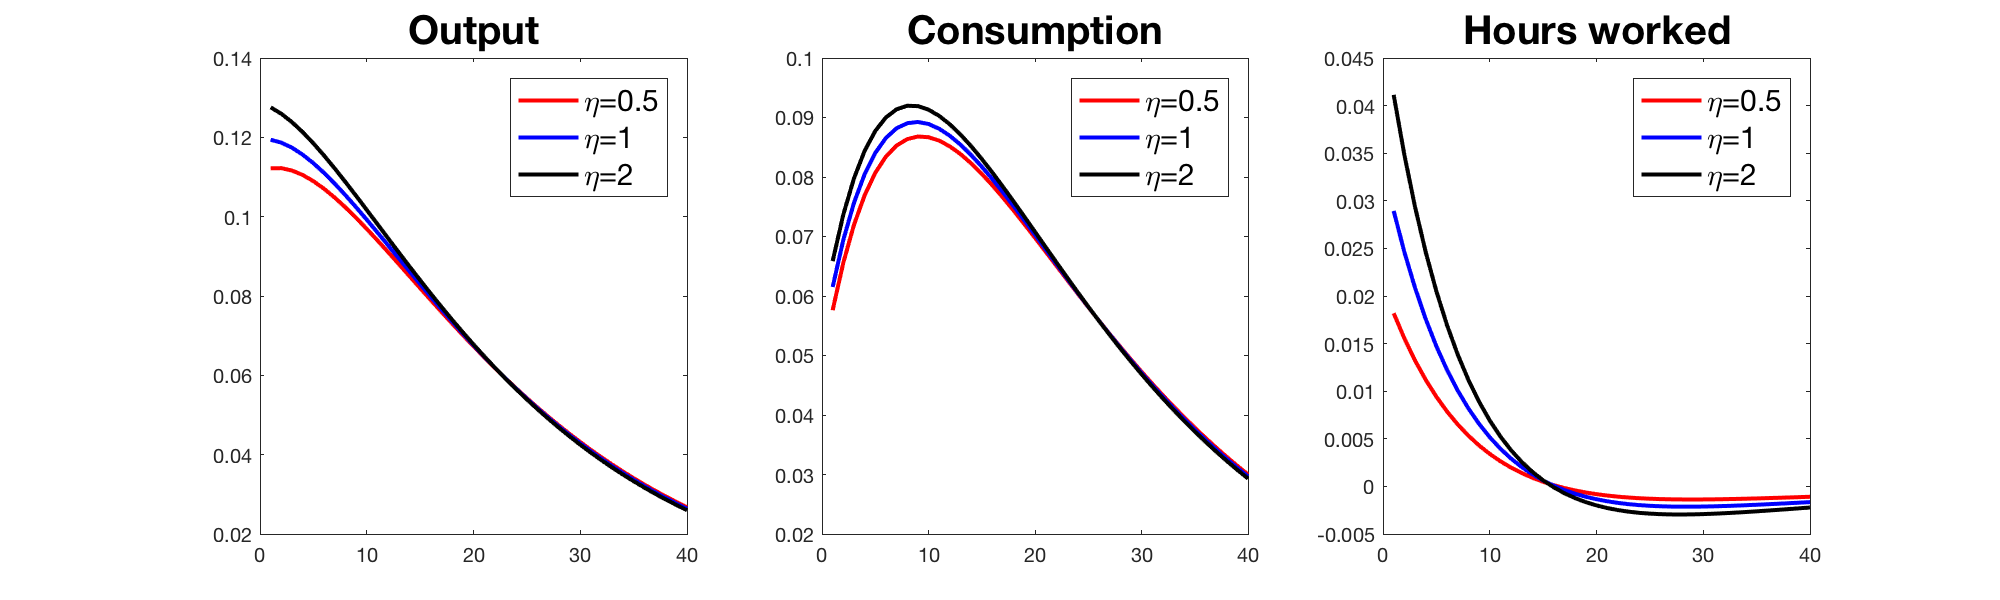
\includegraphics[width=\textwidth]{Q1}
	\caption{Impulse responses with varying $\eta$}
\end{figure}

\begin{table}[H]
	\centering
	\begin{tabular}{ccccc}
		\hline \hline 
		& $\eta=0.5$  & $\eta = 1$          & $\eta = 2$ & Data  \\
		\hline 
		$Stdev(Y)$ &  1.54    & 1.64    & 1.74    & 1.72     \\
		$Stdev(C)$ &  0.97    & 1.02   & 1.08       & 1.27 \\
		$Stdev(L)$ &   0.23   &  0.37   & 0.53     &  1.59 \\
		\hline
	\end{tabular}
	\caption{Response to a transitory discount factor shock}
\end{table}
As one would expect, the fits get better as we calibrate the Frisch elasticity to bigger values. A large Frisch elasticity generates stronger intertemporal substitution of labor suppply, and hence amplifies the effect of shocks. However, even with a large Frisch elasticity, consumption is too smooth, and the volatility of hours generated from the model falls short of the empirical counterpart. 

\section{Variable capital utilization in an RBC model}
\begin{enumerate}[label=(\alph*)]
	\item The Lagrangian of the firm's profit maximization problem is: 
	\begin{dmath*}
	\mathcal{L} = \mathbb{E}_t \sum_{s} \left( \prod_{k=1}^{s} \left(1 + R_{t+k} \right) \right)^{-1} \times \left[  \left( U_{t+s} K_{t+s-1}  \right)^{\alpha} \left(Z_{t+s} N_{t+s}  \right)^{1-\alpha}  - W_{t+s} N_{t+s} - I_{t+s} + q_{t+s} \left( -K_{t+s} + (1-\delta(U_t))K_{t+s-1} + I_{t+s} \right) \right] 
	\end{dmath*}
	The first order conditions are: 
	
	\begin{align*}
	\frac{\partial \mathcal{L}}{\partial N_{t}} : \quad & W_{t} = (1-\alpha) \frac{Y_t}{N_t} \\
	\frac{\partial \mathcal{L}}{\partial I_{t}} : \quad & q_t = 1 \\
	\frac{\partial \mathcal{L}}{\partial K_{t}} : \quad & q_t = \mathbb{E}_t \frac{1}{1 + R_{t+1}} \left[ \alpha \left( U_{t+1} K_{t}  \right)^{\alpha-1} U_{t+1} \left(Z_{t+1} N_{t+1}  \right)^{1-\alpha}  + q_{t+1} \left( 1-\delta(U_{t+1}) \right) \right] \\
		\frac{\partial \mathcal{L}}{\partial U_{t}} : \quad & q_t \delta^{'}(U_t) K_{t-1}  = \alpha \frac{Y_t}{U_t}
	\end{align*}
	
	Combining the second and the third equations, we get the expression for the rental rate of capital. 
	\begin{equation*}
	R_{t+1} = \alpha U_{t+1}^{\alpha} K_{t}^{\alpha-1}  \left(Z_{t+1} N_{t+1}  \right)^{1-\alpha} - \delta(U_{t+1})
	\end{equation*}
	The rental rate depends on $U_t$ because both $MPK$ and depreciation rates depend on $U_t$. 
	
	\item Log linearized version of $q_t \delta^{'}(U_t) K_{t-1}  = \alpha U_t^{\alpha -1} K_{t-1}^\alpha \left( Z_t N_t \right)^{1-\alpha}$ is
	\begin{align*}
	&\check{q_t}+ \frac{\delta^{''}(\bar{U}) \bar{U}}{\delta^{'}(\bar{U})} \check{U}_t + \check{K}_{t-1} = (\alpha -1) \check{U_t} + \alpha \check{K_{t-1}}  + (1-\alpha) \left(  \check{Z_t} + \check{N_t}\right) 
	\end{align*}
	Using $\check{q_t}=0$ and $\check{Y_t} = \alpha \left( \check{U_t} + \check{K_{t-1}} \right) + (1-\alpha) \left(  \check{Z_t} + \check{N_t}\right)$, we can express $\check{U_t}$ in terms of $\check{Y_t}, \check{K_t}$, and $\Delta$. 
	\begin{align*}
	\check{U_t} = \frac{1}{1 + \Delta} \left( \check{Y_t} - \check{K_{t-1}}\right)
	\end{align*}
	
	\item The production function in a log-linear form is: 
	\begin{align*}
	\check{Y_t} &= \alpha \left( \check{U_t} + \check{K_{t-1}} \right) + (1-\alpha) \left(  \check{Z_t} + \check{N_t}\right) \\
	& = \frac{\alpha}{1 + \Delta} \left( \check{Y_t} - \check{K_{t-1}} \right) + \alpha \check{K_{t-1}} + (1-\alpha ) \left(  \check{Z_t} + \check{N_t}\right)
	\end{align*} 
	Isolate $\check{Y_t}$:
	\begin{align*}
	\check{Y_t} &= \frac{\Delta \alpha }{1 + \Delta - \alpha} \check{K_{t-1}} + \frac{(1+\Delta)(1-\alpha)}{1+ \Delta - \alpha} \left(  \check{Z_t} + \check{N_t} \right)  \\
	& = \check{Z_t} + \check{N_t} \quad \left( \text{when } \Delta = 0 \right) \\
	& = \alpha \check{K_{t-1}} + (1-\alpha) \left( \check{Z_t } + \check{N_t} \right)   \quad \left( \text{when } \Delta = \infty \right)
	\end{align*}
	\begin{enumerate}[label = (\roman*)]
    \item $\Delta = 0 $ means that the steady state capital utilization rate is zero. Hence no matter how big the capital stock is, it does not contribute to the output. Therefore, deviations of output from its steady state solely depend on technology and labor. 
    
    \item $\Delta = \infty$ means that steady state capital utilization rate is one. In this case, this model boils down to a model without capital utilization, since 100\% of capital stock is always used in production. Therefore, deviations of output from its steady state depend on all three inputs of the production function, with weights corresponding to the inputs same as the Cobb-Douglas coefficients. 
    
    \item Consider the case when $0 < \Delta < \infty$. In this case, the log linearized production function is written as: 
    \begin{equation*}
    \check{Y_t} = \frac{\Delta \alpha }{1 + \Delta - \alpha} \check{K_{t-1}} + (1-\alpha) \left( \check{Z_t} + \check{N_t} \right)+ \frac{\alpha (1-\alpha)}{1+ \Delta - \alpha} \left(  \check{Z_t} + \check{N_t} \right)
    \end{equation*}
    Since capital stock is not fully used in production, the contributions of $Z_t$ and $N_t$ in $Y_t$ is higher than when $\Delta = \infty$. 
    \end{enumerate}
    \item Since the labor demand curve is downward sloping, to attain indeterminacy we need a downward sloping labor supply curve. Household's labor supply curve is: 
    \begin{equation*}
    L_t = W_t^{\frac{1}{\chi}}
    \end{equation*}
    Hence, negative value of $\chi$ is needed to make the labor supply curve downward sloping. Therefore, with $\chi >0$ assumption, it is impossible to make indeteminacy by adjusting $\chi$. 
    
    We can also check if it's possible to attain a downward-sloping labor demand curve. The linearized labor demand function is $\check W_t = \check Y_t - \check N_t$. Substituting the expression for $\check Y_t$,
    
    $$ \check W_t =  \frac{\Delta \alpha }{1 + \Delta - \alpha} \check{K_{t-1}} + \frac{(1+\Delta)(1-\alpha)}{1+ \Delta - \alpha} \left(  \check{Z_t} + \check{N_t} \right) - \check N_t $$
    
    We can obtain an upward sloping labor demand function if labor exhibits increasing returns to scale, which is when the following condition is satisfied:
    \begin{align*}
    &\frac{(1+\Delta)(1-\alpha)}{1+ \Delta - \alpha} > 1  \\
    \rightarrow & \frac{-\Delta \alpha}{1 + \Delta - \alpha } > 0 
    \end{align*}
    Since $\Delta, \alpha > 0$, indeterminacy is only possible when $1 + \Delta < \alpha$. Hence, with a Cobb-Douglas production function with $0 < \alpha < 1$, indeterminacy is impossible in this model.  
\end{enumerate}

\section{Homework in macroeconomics}
\begin{enumerate}[label = (\alph*)]
	\item The Lagrangian for the household's maximization problem is:
	\begin{equation*}
	\mathcal{L} = \left( C_m^\rho + C_h^\rho \right)^{\frac{1}{\rho}} - \left( \frac{1}{\eta} + 1 \right)^{-1} \left(  L_h + L_m \right)^{\frac{1}{\eta} + 1} + \lambda \left( W L_m - C_m \right) + \xi \left(L_h - C_h \right)
	\end{equation*}
	The first order conditions for the interior solutions are:
	\begin{align*}
	\left( C_m^\rho + C_h^\rho \right)^{\frac{1}{\rho} -1} C_m^{\rho-1} &= \lambda \\
	\left( C_m^\rho + C_h^\rho \right)^{\frac{1}{\rho} -1} C_h^{\rho-1} & = \xi \\
	\left(  L_h + L_m \right)^{\frac{1}{\eta} }  &=\lambda W \\
	\left(  L_h + L_m \right)^{\frac{1}{\eta} }  &= \xi 	 
	\end{align*}
	\item $\xi = \lambda W $
	\item $\xi = \lambda \left( \frac{C_m}{C_h} \right)^{1-\rho}$ \\
	\item Assuming an interior solution, $C_h = L_h = C_m W^{\frac{1}{\rho-1}}$
	\item Combining $L_h = C_h = C_m W^{\frac{1}{\rho-1}}$ and $C_m = W L_m$, we get $L_h = L_m W^{\frac{\rho}{\rho-1}}$. Substituting this into $\left(  L_h + L_m \right)^{\frac{1}{\eta} }  =\lambda W$, we get:
	\begin{equation*}
	L_m \left( 1 + W^{\frac{\rho}{\rho-1}} \right) = \left( \lambda W \right)^\eta
	\end{equation*}
	Hence, 
	\begin{equation*}
	L_m = \frac{(\lambda W)^\eta}{1 + W^{\frac{\rho}{\rho-1}}}
	\end{equation*}
	
	\item Differentiate $L_m$ with respect to $W$:
	\begin{equation*}
	\frac{\partial L_h}{\partial W} = \frac{(1 + W^{\frac{\rho}{\rho-1}}) \lambda^{\eta} \eta W^{\eta - 1} - (\lambda W)^{\eta} (\frac{\rho}{\rho-1}) W^{\frac{\rho}{\rho-1} - 1}}{(1 + W^{\frac{\rho}{\rho-1}})^2}
	\end{equation*}
	Hence the elasticity of $L_m$ with respect to $W$ is: 
	\begin{align*}
	\varepsilon_{L_m,W} = \frac{\partial L_m}{\partial W} \cdot \frac{W}{L_m} &= \frac{(1 + W^{\frac{\rho}{\rho-1}}) \eta  -  (\frac{\rho}{\rho-1}) W^{\frac{\rho}{\rho-1}}}{(1 + W^{\frac{\rho}{\rho-1}})} \\
	&= \eta + \left( \frac{\rho}{1-\rho} \right) \left( \frac{W^{\frac{\rho}{\rho-1}}}{1 + W^{\frac{\rho}{\rho-1}}} \right) 
	\end{align*}
	
	\item Consider a case where $\rho \rightarrow 1$ ($C_m$ and $C_h$ being perfect substitutes). Then, $\frac{\rho}{1 - \rho} \rightarrow \infty$, pushing up the Frisch elasticity to infinity. Intuitively, if the household can home-produce everything on the market, there is no reason to supply labor to the market when the wage is lower than the value of the home produced goods. 
	
	As $\rho$ gets smaller, the Frisch elasticity also approaches to $\eta$. If home produced goods and goods on the market are not substitutable, then the Frisch elasticity is exactly equals to $\eta$. 
	
	\item
	From the first order condition for market consumption goods, we had
	\[
	\left( C_m^\rho + C_h^\rho \right)^{\frac{1}{\rho} -1}  C_m^{\rho-1} = \lambda
	\]
	Assuming interior solutions, substitute the budget constraints
	\[
	((W L_m)^{\rho} + L_h^{\rho})^{\frac{1}{\rho} -1} (W L_m)^{\rho-1} = \lambda
	\]
	and use the substitution
	\[
	L_h = L_m W^{\frac{\rho}{\rho-1}}
	\]
	to get
	\[
	((W L_m)^{\rho} + ( W^{\frac{\rho^2}{\rho-1}}) L_m^{\rho})^{\frac{1}{\rho} -1} (W L_m)^{\rho-1} = \lambda
	\]
	so now substitute back in to
	\[
	L_m = \frac{(\lambda W)^{\eta}}{(1 + W^{\frac{\rho}{\rho-1}})}
	\]
	and we have
	\[
	L_m = \frac{ \left[((W L_m)^{\rho} + ( W^{\frac{\rho^2}{\rho-1}}) L_m^{\rho})^{\frac{1}{\rho} -1} (W L_m)^{\rho-1}\right]^{\eta} W^{\eta}}{(1 + W^{\frac{\rho}{\rho-1}})}
	\]
	and we can simplify to get
	\[
	L_m = \frac{ \left[((W^{\rho} + W^{\frac{\rho^2}{\rho-1}}) L_m^{\rho})^{\frac{1}{\rho} -1} (W L_m)^{\rho-1}\right]^{\eta} W^{\eta}}{(1 + W^{\frac{\rho}{\rho-1}})}
	\]
	and again to get
	\[
	L_m = \frac{ \left[(W^{\rho} + W^{\frac{\rho^2}{\rho-1}})^{\frac{1}{\rho} -1} L_m^{1-\rho} (W L_m)^{\rho-1}\right]^{\eta} W^{\eta}}{(1 + W^{\frac{\rho}{\rho-1}})}
	\]
	and the $L_m$ terms on the right side cancel so we have
	\[
	L_m = \frac{ \left[(W^{\rho} + W^{\frac{\rho^2}{\rho-1}})^{\frac{1}{\rho} -1}  W ^{\rho-1}\right]^{\eta} W^{\eta}}{(1 + W^{\frac{\rho}{\rho-1}})}
	\]
	Simplify this a little bit more:
	\begin{equation*}
	L_m = \left( 1 + W^{\frac{\rho}{\rho-1}} \right)^{\eta \left( \frac{1-\rho}{\rho} \right) -1} W^\eta
	\end{equation*}
	Differentiate $L_m$ w.r.t $W$
	\begin{dmath*}
	\frac{\partial L_m}{\partial W} = \eta W^{\eta -1 } \left( 1 + W^{\frac{\rho}{\rho-1}} \right)^{\eta \left( \frac{1-\rho}{\rho} \right) -1} + W^\eta \left( \eta \left( \frac{1-\rho}{\rho} \right) -1  \right)  \left( 1 + W^{\frac{\rho}{\rho-1}} \right)^{\eta \left( \frac{1-\rho}{\rho} \right) -2} \left( \frac{\rho}{\rho-1} \right) W^{\frac{1}{\rho-1}}
	\end{dmath*}
	Hence the elasticity of $L_m$ w.r.t $W$ is
	\begin{align*}
	\frac{\partial L_m}{\partial W} \frac{W}{L_m} &= \eta + \left( \eta \left( \frac{1-\rho}{\rho} \right) -1  \right) \left( \frac{\rho}{\rho-1} \right) \frac{W^{\frac{\rho}{\rho-1}}}{1 + W^{\frac{\rho}{\rho-1}}} \\
	& = \eta + \left(  \frac{\rho}{1-\rho} - \eta \right) \frac{W^{\frac{\rho}{\rho-1}}}{1 + W^{\frac{\rho}{\rho-1}}} \\
	& =  \eta + \left( \frac{\rho}{1-\rho} \right) \left( \frac{W^{\frac{\rho}{\rho-1}}}{1 + W^{\frac{\rho}{\rho-1}}} \right) - \eta \left(  \frac{W^{\frac{\rho}{\rho-1}}}{1 + W^{\frac{\rho}{\rho-1}}}  \right)
	\end{align*}
	\item The Frisch elasticity of labor measures the percentage change in hours worked due to the percentage change in wages, holding constant the marginal utility of wealth. This implies that the Frisch elasticity of $L_m$ in our model is expressed as:
    \begin{equation*}
    \varepsilon_{L_m, W} \big|_{\lambda = \bar{\lambda}} = \frac{\partial L_m}{\partial W} \cdot \frac{W}{L_m} \big|_{\lambda = \bar{\lambda}}
    \end{equation*}
    This is what we derived in (h). In other words, the Frisch elasticity is the compensated labor elasticity of wage. However, if calculate the Frisch elasticity of $L_m$ holding the total consumption level $C$ as constant, we have 
    \begin{align*}
    \varepsilon_{L_m, W}\big|_{C = \bar{C}} &= \eta + \left( \frac{\rho}{1-\rho} \right) \left( \frac{W^{\frac{\rho}{\rho-1}}}{1 + W^{\frac{\rho}{\rho-1}}} \right) - \eta \left(  \frac{W^{\frac{\rho}{\rho-1}}}{1 + W^{\frac{\rho}{\rho-1}}}  \right) \\
    & = \varepsilon_{L_m, W} \big|_{\lambda = \bar{\lambda}} - \eta \left(  \frac{W^{\frac{\rho}{\rho-1}}}{1 + W^{\frac{\rho}{\rho-1}}}  \right)
    \end{align*}
    The last negative term represents the wealth effect from the rise in $W$, since we are not holding the wealth effect constant in this case. However, the intuition from (g) still survives. 
    
	\item Even if $\eta$ itself is small, the model can generate a high Frisch elasticitiy by adjusting the substitutability parameter $\rho$. If home produced and market produced goods are highly substitutable, households would want to move their labor almost entirely from the home production to the labor market. This induces a high Frisch elasticity regardless of the value of $\eta$. 

\end{enumerate}

\section{$q$-Theory with Variable Capital Utilization}
\begin{enumerate}[label = (\alph*)]
	\item The Lagrangian of the firm's profit maximization problem is: 
	\begin{align*}
	\mathcal{L} =& \mathbb{E}_t \sum_{s} \left( \prod_{k=1}^{s} \left(1 + r_{t+k} \right) \right)^{-1} \\
	\begin{split}
	&\times \left\lgroup  Z_{t+s} \left( U_{t+s} K_{t+s-1}  \right)^{\alpha} L_{t+s}^{1-\alpha}  - W_{t+s} L_{t+s} - I_{t+s} \left[ 1 + \phi \left( \frac{I_{t+s}}{K_{t+s-1}} \right) \right] \right. \\
	& \qquad + q_{t+s} \left( -K_{t+s} + (1-\delta(U_t))K_{t+s-1} + I_{t+s} \right) \left. \right\rgroup
	\end{split}
	\end{align*}
	This problem is truly dynamic because the presence of an adjustment cost links the present and future period investment decisions. 
	\item The first order conditions are: 
	\begin{align*}
		\frac{\partial \mathcal{L}}{\partial L_t}: &\quad  w_t = (1-\alpha) \frac{Y_t}{L_t} \\
		\frac{\partial \mathcal{L}}{\partial L_t}: & \quad q_t = 1 + \phi \bigg ( \frac{I_t}{K_t} \bigg ) + \frac{I_t}{K_t} \phi' \bigg ( \frac{I_t}{K_t} \bigg ) \\
		\frac{\partial \mathcal{L}}{\partial K_t}: & \quad q_t = (1+r_{t+1})^{-1} \bigg ( \alpha \frac{Y_{t+1}}{K_{t+1}} + \frac{I_{t+1}^2}{K_{t+1}^2} \phi' \bigg ( \frac{I_t}{K_t} \bigg ) + q_{t+1} (1-\delta(U_{t+1})) \bigg ) \\
		\frac{\partial \mathcal{L}}{\partial U_t}: &\quad  \alpha \frac{Y_t}{U_t} = q_t \delta'(U_t) K_t
	\end{align*}
	Combining the second and third equations, we can get an expression for the rental rate of capital: 
	\begin{equation*}
	r_{t+1} = \alpha \frac{Y_{t+1}}{K_{t+1}} + \frac{I_{t+1}^2}{K_{t+1}^2} \phi' \bigg ( \frac{I_t}{K_t} \bigg )  + \delta(U_{t+1})
	\end{equation*}
	The rental rate of captial is a function of $U$ because the depreciation rate and the marginal product of capital depend on $U$. It is also a function of $q$ because -
	
	\item Log-linearized version of the FOC for utilization is:
	\begin{align*}
	\check U_t = \frac{\check Y_t  - \check K_t - \check q_t}{1 + \Delta} = \frac{\check{MPK}_t - \check q_t}{1 + \Delta} \\
	\end{align*}
	Hence the sign of the percentage deviation of utilization from its steady state value depends on $\check MPK_t - \check q_t$. In this model, $q_t$ can be different from 1. Considering that $q_t$ is a Lagrangian multiplier attached to the capital accumulation equation, the interpretation of $q_t$ is \textit{Tobin's marginal q}, which is the ratio of the value of additional unit of capital to its replacement cost. Hence, $\check MPK_t - \check q_t$ represents the net gain of adding one more unit of capital in the production. When $\check MPK_t - \check q_t > 0$, it is profitable for the firm to use more units of capital, hence $\check U_t >0$. 
	
	\item In this model, capital utilization is negatively correlated with $q$. Since $q$ and investment are positively correlated, procyclical investment implies counter-cyclical utilization. However, this statement is not unambiguously true because $MPK$ can also be procyclical. 
	
	\item To make the argument less complicated, I rule out the impact of the shock to labor. Consider a permanent (or a highly persistent) shock to $Z$. When the shock is expected to be permanent or prolonged for a long period of time, firms react by building up more capitals. This implies that $\check{MPK} <0$. Hence, for a highly persistent shock, $U_t$ is countercyclical. Since higher utilization induces higher depreciation rate, it is better to reduce the utilization rate once the firm decides to build up additional capital stock. 
	
	However, when the shock is merely transitory, firms would not want to build up more capital, because those additional capital stock will be excessive when the shock disappears. This means that $\check{MPK} >0$. Hence, there is a possibility that $U_t$ can be procyclical when the shock is transitory. 
	
	In short, firms react to a transitory shock by using the existing amount of capital more intensively. When faced with a permanent or highly persistent shock, firms would rather decide to build up more capital rather than using the current capital stock more intensively. 
\end{enumerate}

\section{Fiscal multiplier in the RBC model}
\begin{enumerate}[label = (\alph*)]
	\item
	The log-linearized system of equations is
	\begin{align*}
		&\check{K}_t = (1-\delta) \check{K}_{t-1} + \delta \check{I}_t \\
		&\check{C}_t + \frac{1}{\eta} \check{L}_t = \check{Y}_t - \check{L}_t \\
		&E_t \check{C}_{t+1} - \check{C}_t = \frac{\alpha \frac{\bar{Y}}{\bar{K}}}{\alpha \frac{\bar{Y}}{\bar{K}} + (1-\delta)} (E_t \check{Y}_{t+1} - \check{K}_t ) \\
		&\check{Y}_t = \alpha \check{K}_{t-1} + (1-\alpha) \check{L}_t \\
		&\check{Y}_t = \frac{\bar{C}}{\bar{Y}} \check{C}_t + \frac{\bar{I}}{\bar{Y}} \check{I}_t + \frac{\bar{G}}{\bar{Y}} \check{G}_t \\
		&\check{G}_t = \rho_g \check{G}_{t-1} + \epsilon_t^g
	\end{align*}
	Guess that the policy functions take the form
	\begin{align*}
		&\check{C}_t = v_{CK} \check{K}_{t-1} + v_{CG} \check{G}_{t} \\
		&\check{K}_t = v_{KK} \check{K}_{t-1} + v_{KG} \check{G}_{t}
	\end{align*}
	Now plug the policy functions into the system of equations and we are left with the log-linearized consumption Euler equation and labor-leisure condition in terms of parameters, coefficients of the policy functions, and state variables:
	\begin{dmath*}
		(v_{CK} v_{KK} - v_{CK}) \check{K}_{t-1} + (v_{CK} v_{KG} + v_{CG}\rho_g - v_{CG}) \check{G}_{t} = \frac{\alpha \frac{\bar{Y}}{\bar{K}}}{\alpha \frac{\bar{Y}}{\bar{K}} + (1-\delta)} \left[ \frac{\bar{C}}{\bar{Y}} v_{CK} v_{KK} + \frac{\bar{I}}{\bar{Y}} (v_{KK} - 1 + \delta) v_{KK} \frac{1}{\delta} - v_{KK} \right] \check{K}_{t-1} + \frac{\alpha \frac{\bar{Y}}{\bar{K}}}{\alpha \frac{\bar{Y}}{\bar{K}} + (1-\delta)} \left[ \frac{\bar{C}}{\bar{Y}} v_{CK} v_{KG} + \frac{\bar{C}}{\bar{Y}} v_{CG} \rho_g + \frac{\bar{I}}{\bar{Y}} (v_{KK} - 1 + \delta) v_{KG} \frac{1}{\delta} + \frac{\bar{I}}{\bar{Y}} v_{KG} \rho_g \frac{1}{\delta} + \frac{\bar{G}}{\bar{Y}} \rho_g - v_{KG} \right] \check{G}_t
	\end{dmath*}
	\begin{dmath*}
		\left[ v_{CK} - \left( \frac{1}{\eta} + 1 \right) \frac{\alpha}{1-\alpha} \right] \check{K}_{t-1} + v_{CG} \check{G}_t = \frac{-\alpha - \frac{1}{\eta}}{1-\alpha} \left[ \frac{\bar{C}}{\bar{Y}} v_{CK} + \frac{\bar{I}}{\bar{Y}} (v_{KK} - 1 + \delta) \frac{1}{\delta} \right] \check{K}_{t-1} + \frac{-\alpha - \frac{1}{\eta}}{1-\alpha} \left[ \frac{\bar{C}}{\bar{Y}} v_{CG} + \frac{\bar{I}}{\bar{Y}} v_{KG} \frac{1}{\delta} + \frac{\bar{G}}{\bar{Y}} \right] \check{G}_{t}
	\end{dmath*}
	By comparing the coefficients on $\check{K}_{t-1}$ and $\check{G}_t$ in both equations, we obtain 4 equations
	\begin{dmath*}
		v_{CK} v_{KK} - v_{CK} = \frac{\alpha \frac{\bar{Y}}{\bar{K}}}{\alpha \frac{\bar{Y}}{\bar{K}} + (1-\delta)} \left[ \frac{\bar{C}}{\bar{Y}} v_{CK} v_{KK} + \frac{\bar{I}}{\bar{Y}} (v_{KK} - 1 + \delta) v_{KK} \frac{1}{\delta} - v_{KK} \right]
	\end{dmath*}
	\begin{dmath*}
		v_{CK} v_{KG} + v_{CG}\rho_g - v_{CG} = \frac{\alpha \frac{\bar{Y}}{\bar{K}}}{\alpha \frac{\bar{Y}}{\bar{K}} + (1-\delta)} \left[ \frac{\bar{C}}{\bar{Y}} v_{CK} v_{KG} + \frac{\bar{C}}{\bar{Y}} v_{CG} \rho_g + \frac{\bar{I}}{\bar{Y}} (v_{KK} - 1 + \delta) v_{KG} \frac{1}{\delta} + \frac{\bar{I}}{\bar{Y}} v_{KG} \rho_g \frac{1}{\delta} + \frac{\bar{G}}{\bar{Y}} \rho_g - v_{KG} \right]
	\end{dmath*}
	\begin{dmath*}
		v_{CK} - \left( \frac{1}{\eta} + 1 \right) \frac{\alpha}{1-\alpha} = \frac{-\alpha - \frac{1}{\eta}}{1-\alpha} \left[ \frac{\bar{C}}{\bar{Y}} v_{CK} + \frac{\bar{I}}{\bar{Y}} (v_{KK} - 1 + \delta) \frac{1}{\delta} \right]
	\end{dmath*}
	\begin{dmath*}
		v_{CG} \check{G}_t = \frac{-\alpha - \frac{1}{\eta}}{1-\alpha} \left[ \frac{\bar{C}}{\bar{Y}} v_{CG} + \frac{\bar{I}}{\bar{Y}} v_{KG} \frac{1}{\delta} + \frac{\bar{G}}{\bar{Y}} \right] \check{G}_{t}
	\end{dmath*}

	\item
	Increase in government expenditure is only temporary, and the boost in output is transitory. Households compensate for the increased government expenditure by decreasing consumption, decreasing savings, and increasing labor supply. The households desired level of steady-state capital remains unchanged. This causes MPL (and wages) to decline while MPK (and interest rate) to increase.

	\item
	The multiplier is about 1.13.

	\item
	Now the increase in government expenditure is permanent, and the boost in output persists forever. Households decrease consumption and increase labor supply by a lot more compared to before because they are increasing their savings in this situation. This is because the households want to attain a higher level of steady-state capital. This sharp increase in labor supply causes wages to decline by more and interest rate to increase more. The level of increase in output is much larger; the multiplier is about 1.4.
\end{enumerate}
\end{document}
